\section{\label{III-C-2}Établir une méthodologie particulière d'alignement}
\titreEntete{Une méthodologie particulière}

%intro
En raison des difficultés identifiées dans la \reference{III-C-1}, un alignement simple, n'apportant aucune indication de fiabilité, n'est pas possible. De même, les alignements réalisés dans les chapitres précédents utilisent chacun les jeux de données initiaux jusqu'à la fin du traitement, sans en retirer au fur et à mesure les concepts qui viennent d'être alignés. L'alignement des référentiels de la \ac{ddcol} et de la \ac{dj} se distingue des précédents par la nécessité d'une méthodologie particulière, basée sur un indice de confiance attribué à chaque alignement, et sur une succession d'étapes, représentant les niveaux de confiance apportés au type de jointure utilisé.

\subsection{\label{III-C-2-a}Créer un indice de confiance pour chaque alignement}
\titreEntete{Créer un indice de confiance}

Les points de contact entre les jeux de données n'ont pas tous la même valeur dans un alignement. En effet, l'état civil d'une personne, bien qu'essentiel dans un alignement, peut conduire à aligner deux homonymes: c'est pourquoi les points de contact comme les noms, les prénoms ou les pseudos peuvent être considérés comme ayant une faible valeur dans le processus d'alignement. De plus, leur octroyer une valeur forte conduirait à surévaluer les alignements réalisés sur la simple comparaison des noms et prénoms sans autre point de comparaison par rapport aux alignements qui n'auront pas été possibles.\\

En revanche, la valeur des points de comparaison significatifs est considérée comme forte: il s'agit de la date de décès ou de la contribution. En effet, la probabilité que les états civils et les dates de décès de deux homonymes soient identiques est très faible, ce qui peut permettre de donner à cet alignement une valeur plus forte. De même, la correspondance entre une contribution et une fonction est considérée comme très fiable quand les états civils ont déjà été rapprochés: pour cette raison, le point de comparaison sur la contribution est celui qui possède l'indice de confiance le plus élevé, puisqu'il est le point le plus spécifique, et le plus difficile à faire correspondre.\\

Enfin, la comparaison du sexe permet également d'augmenter la fiabilité d'un alignement. Dans la majorité des alignements réalisés, la comparaison peut sembler évidente à l'humain, mais dans certains cas, comme pour les prénoms \textit{Dominique}, elle est nécessaire et permet la conservation ou non de l'alignement.\\

L'indice de confiance permet une priorisation des points de comparaison, une hiérarchisation de ces derniers. Il se forme à partir de la somme des scores de chaque point de comparaison. Ainsi, dans le cas de l'alignement des référentiels de personnes de la \ac{dj} et de la \ac{ddcol}, l'indice de confiance varie entre 0 --- quand l'alignement n'a pas pu être réalisé --- et 9 --- quand tous les points de comparaison ont été réalisés avec succès --- selon les scores de la \reference{table_scores}.
\begin{table}[!h]
	\centering
	\begin{tabular}{|c|c|}
		\hline
		\textbf{Point de comparaison}&\textbf{Score}\\ \hline
		Nom&1\\ \hline
		Prénom&1\\ \hline
		Pseudo nom&1\\ \hline
		Pseudo prénom&1\\ \hline
		Sexe&1\\ \hline
		Date de décès&2\\ \hline
		Contribution&2\\ \hline
	\end{tabular}
	\caption{Scores attribués à chaque point de comparaison}
	\label{table_scores}
\end{table}

\subsection{\label{III-C-2-b}Des étapes exclusives}
\titreEntete{Des étapes exclusives}

L'attribution d'un indice de confiance ne permet de résoudre que la problématique de l'évaluation finale des alignements. Il subsiste néanmoins une seconde problématique, celle de la présence, dans les alignements réalisés, de doublons, c'est à dire de personnes de la \ac{dj} alignées avec plusieurs concepts. Une solution pourrait être alors de supprimer les alignements présents. Or, un tel cas est fréquent: supprimer les alignements concernés réduirait la quantité de résultats finaux.\\

Ainsi, après une première priorisation des points de comparaison, il est nécessaire d'effectuer ensuite une priorisation des combinaisons de ces points de comparaison. Quatre étapes principales ont été identifiées.

\noindent D'abord, les alignements réalisés avec le nom, le prénom, les pseudos et la correspondance des fonctions sont considérés comme ceux étant les plus sûrs pour effectuer les rapprochements entre les concepts de la \ac{ddcol} et les matricules de la \ac{dj}. Ces alignements, comme ceux des étapes suivantes, sont des jointures\footnote{Afin de ne récupérer que les alignements qui ont été réalisés, ces jointures sont de type \textit{inner join}.} entre les deux jeux de données réalisées dans l'ETL Talend avec le composant associé, un tMap (\reference{tmap_jointures}).
\begin{figure}[!h]
	\centering
	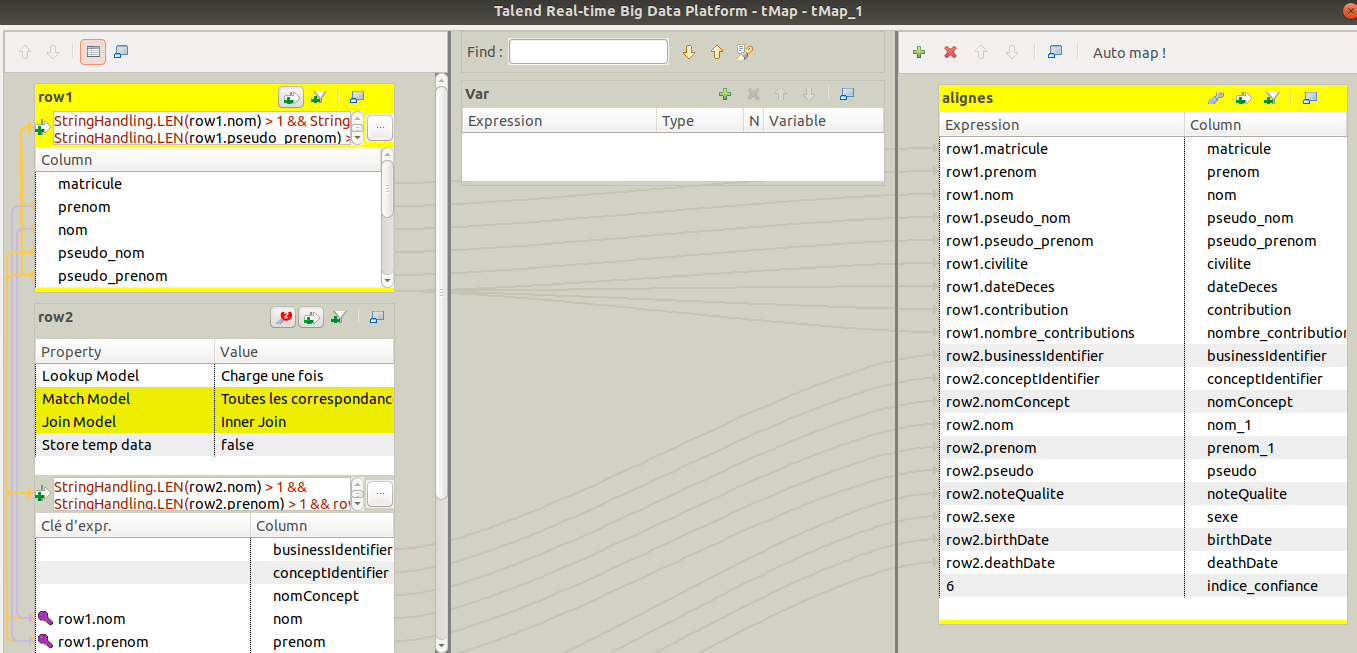
\includegraphics[width=16cm]{images/tmpa_jointure1_dj.png}
	\caption{L'alignement des personnes de la \ac{dj} et de la \ac{ddcol} pour une jointure dans un tMap de Talend.}
	\label{tmap_jointures}
\end{figure}

\noindent Ensuite, les alignements effectués avec le nom, le prénom et les pseudos, sans avoir pu faire correspondre les fonctions, constituent la seconde étape.

\noindent La troisième étape, comme la quatrième, tente de rapprocher deux personnes en prenant en compte les différences de graphie qui peuvent exister. Ainsi, les alignements sont réalisés sur les pseudos, et sur le prénom de la \ac{dj} commençant par le prénom de la \ac{ddcol}\footnote{Une exception a été créé dans cette étape pour les prénoms \textit{Jean} et \textit{Anne}.}. Cette étape permet l'alignement d'une même personne ayant à la \ac{ddcol} le prénom \textit{Louis} et à la \ac{dj} le prénom \textit{Louis Marie}.

\noindent Enfin, l'ensemble des combinaisons possibles étant couvert, il est nécessaire d'effectuer une dernière étape pour réaliser non pas des alignements fiables --- ce qui est le but des trois premières étapes --- mais des alignements permettant d'apporter une aide à un opérateur humain, en proposant plusieurs concepts pouvant être alignés avec un matricule. Ce rapprochement particulier, réalisé sur les seuls nom et prénom, autorise par conséquent la présence de plusieurs concepts alignés avec un même matricule, notamment dans le cas d'homonymes.\\

Distinguer ces quatre étapes permet, à l'issue de chacune d'elles, de récupérer ce qui n'a pas été aligné, tant du côté de la \ac{dj} ou de la \ac{ddcol}, afin d'effectuer l'étape suivante avec uniquement ces données non alignées (\reference{orchestration}). Cette récupération évite de créer des alignements doubles avec des concepts différents entre les étapes. C'est également à l'issue de cette récupération que les résultats des jointures précédentes sont comparés pour supprimer les matricules alignés plusieurs fois, et attribuer les scores pour le sexe et la date.\\
\begin{figure}[!h]
	\centering
	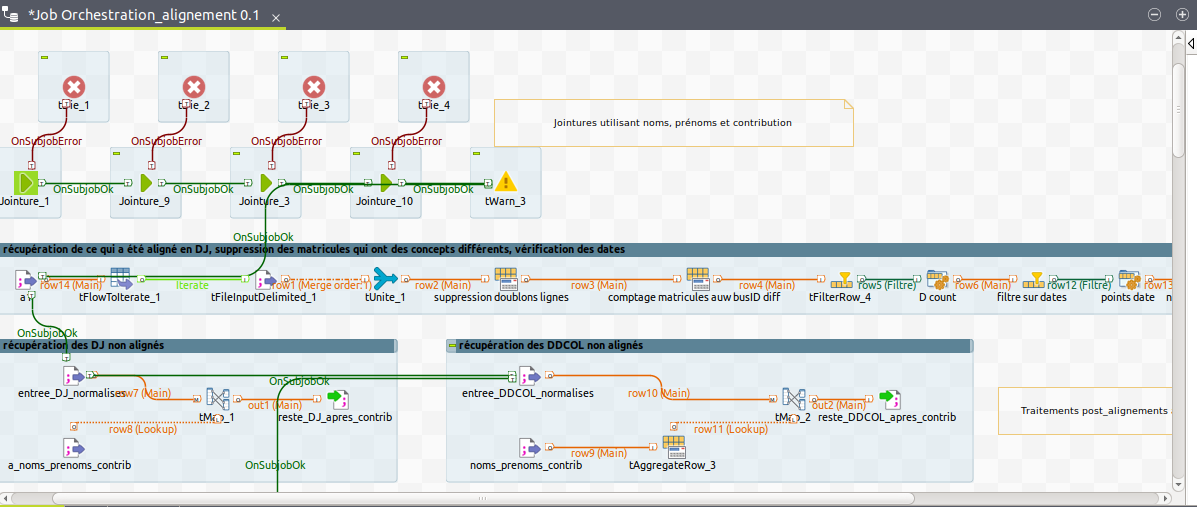
\includegraphics[width=16cm]{images/orchestration_partie1_dj.png}
	\caption{L'orchestration de la première étape dans l'ETL Talend.}
	\label{orchestration}
\end{figure}

Cependant, la limite de la récupération des matricules des personnes non alignées de la \ac{dj} et de la \ac{ddcol} est dans la priorisation ce ces étapes. En effet, elle se base uniquement sur des critères définis en amont par un humain, selon l'observation des cas généraux d'alignements: bien que ce soit une méthode apportant de la fiabilité aux alignements, cette fiabilité n'est pas nécessairement celle qui est la plus optimale. De même, cette récupération pourrait avoir lieu après chaque alignement de matricule: cela ajouterait néanmoins une nouvelle priorisation, basée sur l'ordre de passage, qui serait plus arbitraire encore, puisque cet ordre de passage des matricules de la \ac{dj} dans le processus d'alignement n'est régi par aucun ordre significatif\footnote{Une base de données relationnelle n'étant pas ordonnée.}.

%conlu
\bigskip
\bigskip
Face aux nombreuses difficultés, l'indice de confiance et la priorisation des étapes permettent de réduire les mauvais alignements et d'apporter une précision sur la fiabilité d'un alignement. Cependant, l'automatisation de ce processus présente des limites comme la définition de règles dirigeant le processus d'alignement. L'alignement des soixante-dix mille matricules de la \ac{dj} et des plus de trois cent mille concepts de la \ac{ddcol} ne peut pas être réalisé sur la base de quelques règles puis être considéré comme fiable.